\paragraph{Definition of probability density function (pdf):}
Let $R_{X}$ be the space of the random variable $X$. The function:
$f:R_{X}\rightarrow \mathbb{R}$ defined by:
\begin{align*}
    f(x) &= \Prob{X=x} \text{ if } X \text{ is discrete.}\\
    f(x) &= \Prob{X\in A}=\Su{A}{{}}f(x)dx \text{ if } X \text{ is continuous, with } A
    \text{ a set of real numbers.}
\end{align*}
is called probability density function of $X$.


\paragraph{Definition of cumulative density function (cdf):}
Let $R_{X}$ be the space of the random variable $X$. The function:
$F:R_{X}\rightarrow \mathbb{R}$ defined by:\\
\begin{align*}
    F(x) &= \Prob{X\leq x} \text{ if } X \text{ is discrete.}\\
    F(x) &= \Prob{X\leq x}=\Su{-\infty}{x}f(t)dt \text{ if } X \text{ is continuous, 
    with } A \text{ a set of real numbers.}
\end{align*}


\paragraph{Percentile for continuous random variables.}
Let $p\in [0;1]$, a $100p^{th}$ percentile of the distribution of a random
variable $X$ is $q\in\mathbb{R}$ satisfying:
\begin{center}
	$\Prob{X\leq q}\leq p$\\
	(Recall that the $F$ is a monotonically increasing function, then it has an 
	inverse $F^{-1}$)\\
	$q = F^{-1}(p)$
\end{center}
A $100p^{th}$ is a measure of location for the probability distribution in
the sense that $q$ divides the distribution of the probability mass into
2 parts, one having probability mass $p$ and other having probability mass
$1-p$
\begin{figure}[H]
	\begin{center}
		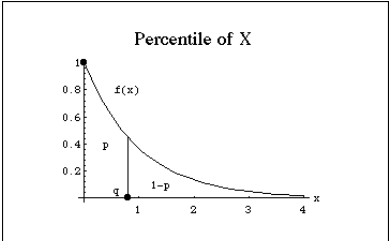
\includegraphics[width=.5\textwidth]{./chapters/2_statistics/01_fundamental_probability_concepts/2_images/1percentile.png}
	\end{center}
	\caption{Percentile}
	\label{fig:fig2.1}
\end{figure}
The $50^{th}$ percentile of any distribution is called median of the distribution.
